To identify settlements in home ranges, the presence of nests and successful broods, an algorithm was developed that treats the three breeding phases separately. In the first part (Section~\ref{subsection:homerange}), individuals were identified that showed ranging behaviour consistent with settling in a home range. In the second part (Section~\ref{subsection:nest}), nest sites are located using recursive movement patterns. In the third part (Section~\ref{subsection:brood_phase_identification}), the phase of incubating the eggs and the phase of feeding the nestlings were defined based on parental movement patterns using an multinomial logistic regression model (MLRM). After the description of the data and the study areas (Section~\ref{subsection:data_study_areas}) and the pre-processing (Section~\ref{subsection:preprocessing}), the three steps of the algorithm are explained in detail. All steps carried out in this work were conducted in the R programming language for statistical computing and graphics in RStudio \parencite{rstudio}.



\subsection{Data and Study Areas}  \label{subsection:data_study_areas}
\subsubsection{Switzerland -- Main Data}
After almost becoming extinct in the 19\textsuperscript{th} and early 20\textsuperscript{th} century, increased numbers of red kite breeding pairs have repopulated the Swiss Plateau strongly, especially since the 1970s. This fact attracted particular attention, as populations in surrounding countries did not increase as much or even stagnated, of which no definite cause can be identified \parencite{swissornithologicalinstitute}. In 2015, the Swiss Ornithological Institute therefore launched a monitoring programme in the Sense region in the cantons of Bern and Fribourg to analyse population dynamics of red kites. The data collected in this project served as the basis for this work. To monitor the red kites, they were equipped with solar-powered GPS transmitters that were attached to their backs. Tagging started in 2015 and was discontinued in 2022. During this period, more than 560 individuals have been equipped with GPS transmitters, accompanied by intensive field work and data analysis. Two different models of GPS transmitters have been used in the project, Ecotone (SKUA/CREX type) since 2015 and Milsar (M9/S9 type) since 2017. While the former model collects location data at an interval of one hour, the latter has a temporal resolution of 10 minutes. In addition to the coordinates, further sensor data are collected, such as timestamp, accelerometry, or temperature. As far as the completeness was guaranteed, data from the entire project duration were used for this work in order to be able to analyse as many breeding cycles as possible. After data pre-processing, movement data of 375 breeding cycles were available, originating from 133 birds from 2016 to 2022.

As background knowledge on the individuals, valuable information was provided by the Swiss Ornithological Institute, which was collected in intensive field work. The area was divided into squares with an edge length of 2.5 kilometres, which were visited at least three times for 1-2 hours each from March to July. Using telescopes and binoculars, the red kites were observed and possibly assigned territories or even nests. Each actively used nest was visited every 1-2 weeks to observe the breeding activity, while most nests were climbed to measure and ring the fledglings and equip them with a GPS transmitter. A blood sample was taken to determine the sex of the fledglings. If the hatching date could not be observed, the age of the fledglings were derived from the weight and the wingspan measurements \parencite{scherler2023brutbiologie}. With this detailed background information, biological characteristics such as sex and age could be assigned to the GPS trajectories. Many individuals could also be assigned a home range or a nest and the timing of egg laying, chick hatching and fledging of nestlings. This information is essential for creating an algorithm to analyse the breeding process and success.

The study area of 387.5 km$^2$ extends from the Central Plateau at 482 metres above sea level to the Pre-Alps at 1763 above sea level \parencite{scherler2023brutbiologie}. The area is shaped by agriculture (56\%), managed forests (27\%), unproductive land (8.5\%) and settlements (8.5\%) \parencite{naegeli2021weather}. The diversely structured landscape with a high proportion of meadows interspersed with forests provides an ideal breeding ground for the red kite \parencite{aebischer2021rotmilan}. Most GPS locations are located in this region and most breeding takes place in this area (Figure~\ref{figure:map_breeding_area}).

\subsubsection{Germany -- Validation Data}
To test the algorithm for its performance in other geographical areas, Thomas Pfeiffer generously provided a dataset of 14 red kites during the years 2016 to 2022, of which 28 breeding cycles of 13 individuals fulfilled the requirements of the algorithm. The data stem from solar-powered GPS transmitters of red kites that bred successfully in Thuringia, Germany (Figure~\ref{figure:map_breeding_area}). Background information was also provided on the sex and timing of egg laying, chick hatching and fledging.

During the breeding season, the birds stay in Thuringia (Figure~\ref{figure:map_breeding_area}). The data points are more concentrated than in the Swiss dataset, which is due to the smaller number of birds tracked. The region in Thuringia, more specifically the Thuringian Basin, has a comparatively more homogeneous landscape structure and a relatively consistent altitude of 200 meters above sea level.

The breeding region in Thuringia, which is located east of Erfurt, lies mainly in the Thuringian Basin, which is at a relatively constant altitude of 130 to 300 metres above sea level, while in the southern part of the breeding region altitudes of over 400 metres above sea level are reached. The area contains the largest area of steppe grassland in Germany and is characterised by a warm dry climate \parencite{baumbach2013steppen}. Due to these conditions, the area is mainly used for agriculture, while there are relatively few forest areas. This landscape characteristic with large open areas leads to relatively large home ranges for red kites, which are significantly larger than for example in the breeding area in Switzerland (Figure~\ref{figure:home_range_diff_ch_de}) studied by the Swiss Ornithological Institute \parencite{aebischer2021rotmilan, pfeiffer2015gps}.

\begin{figure}[H]
\centering
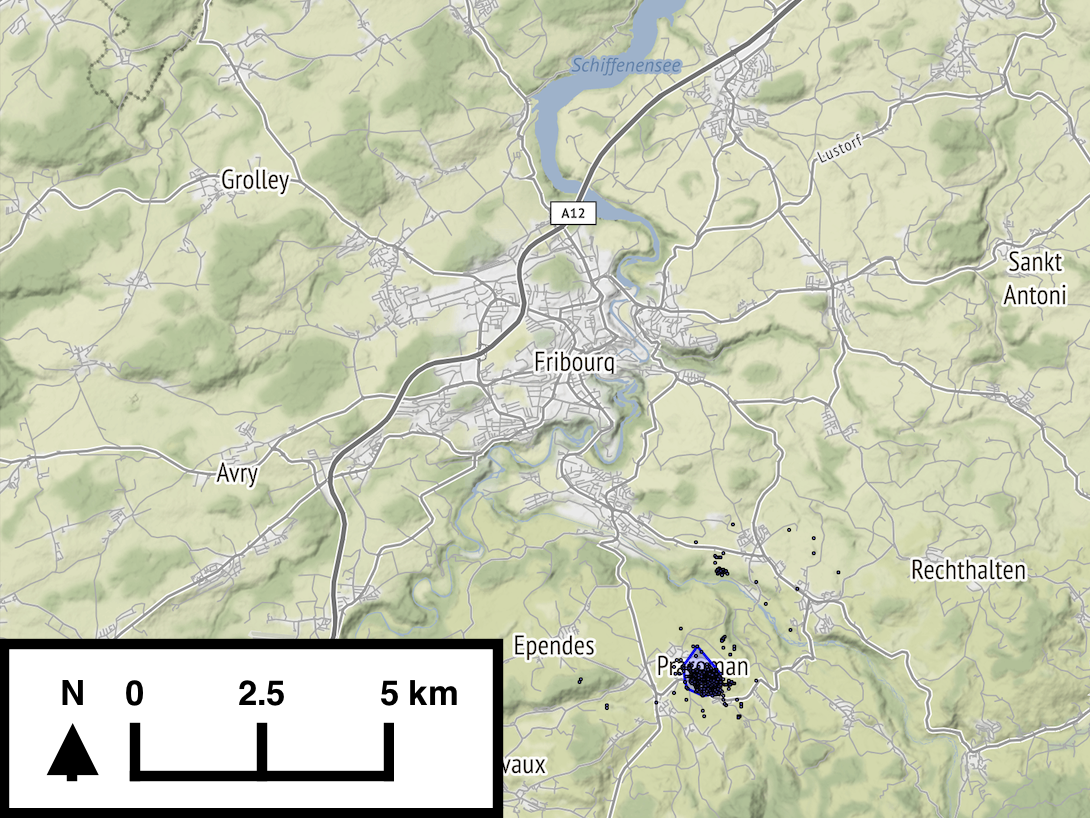
\includegraphics[width=0.495\textwidth]{figures/maps/CH_f_2022.png}
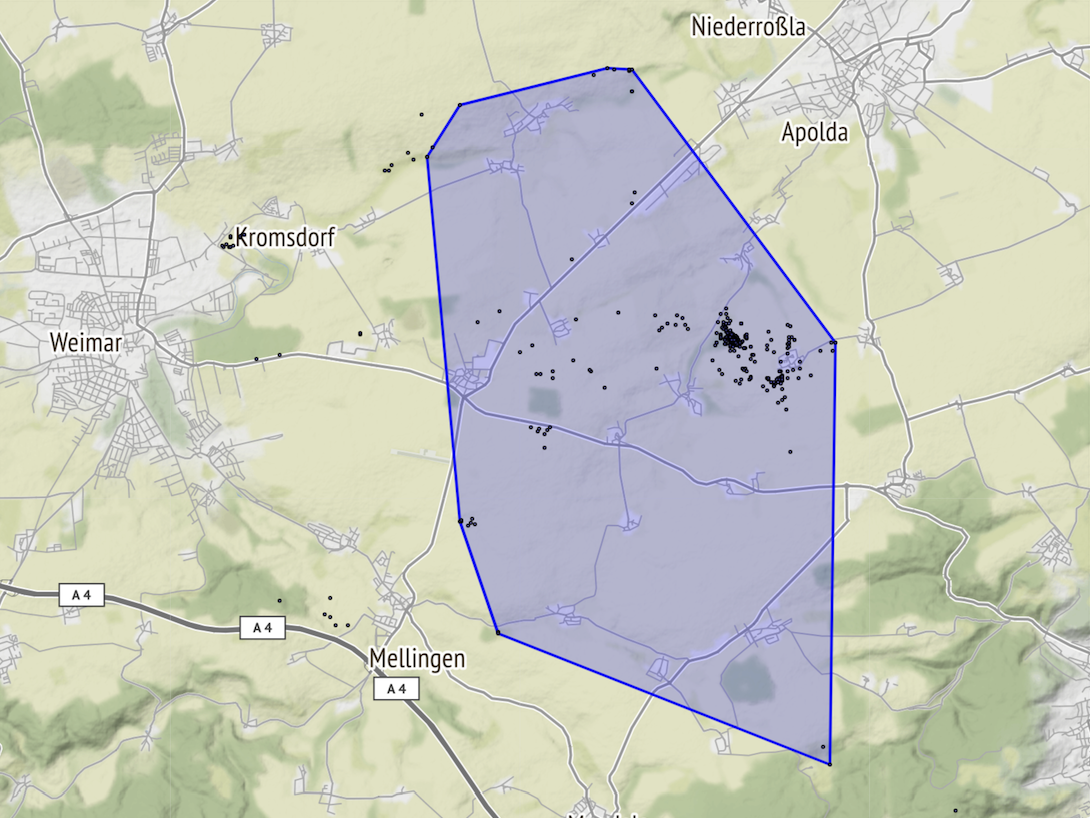
\includegraphics[width=0.495\textwidth]{figures/maps/DE_f_2022.png}
\caption[Comparison of home range sizes in Switzerland and Germany]{Home range sizes (95\% MCP) of female red kites during the breeding season 2022 in Switzerland (left) and in Germany (right). The blue areas represent the home ranges while the black points represent the GPS locations during the breeding cycle. Both maps have the same scale. Base map: Stamen.}
\label{figure:home_range_diff_ch_de}
\end{figure}

\begin{figure}[H]
\centering
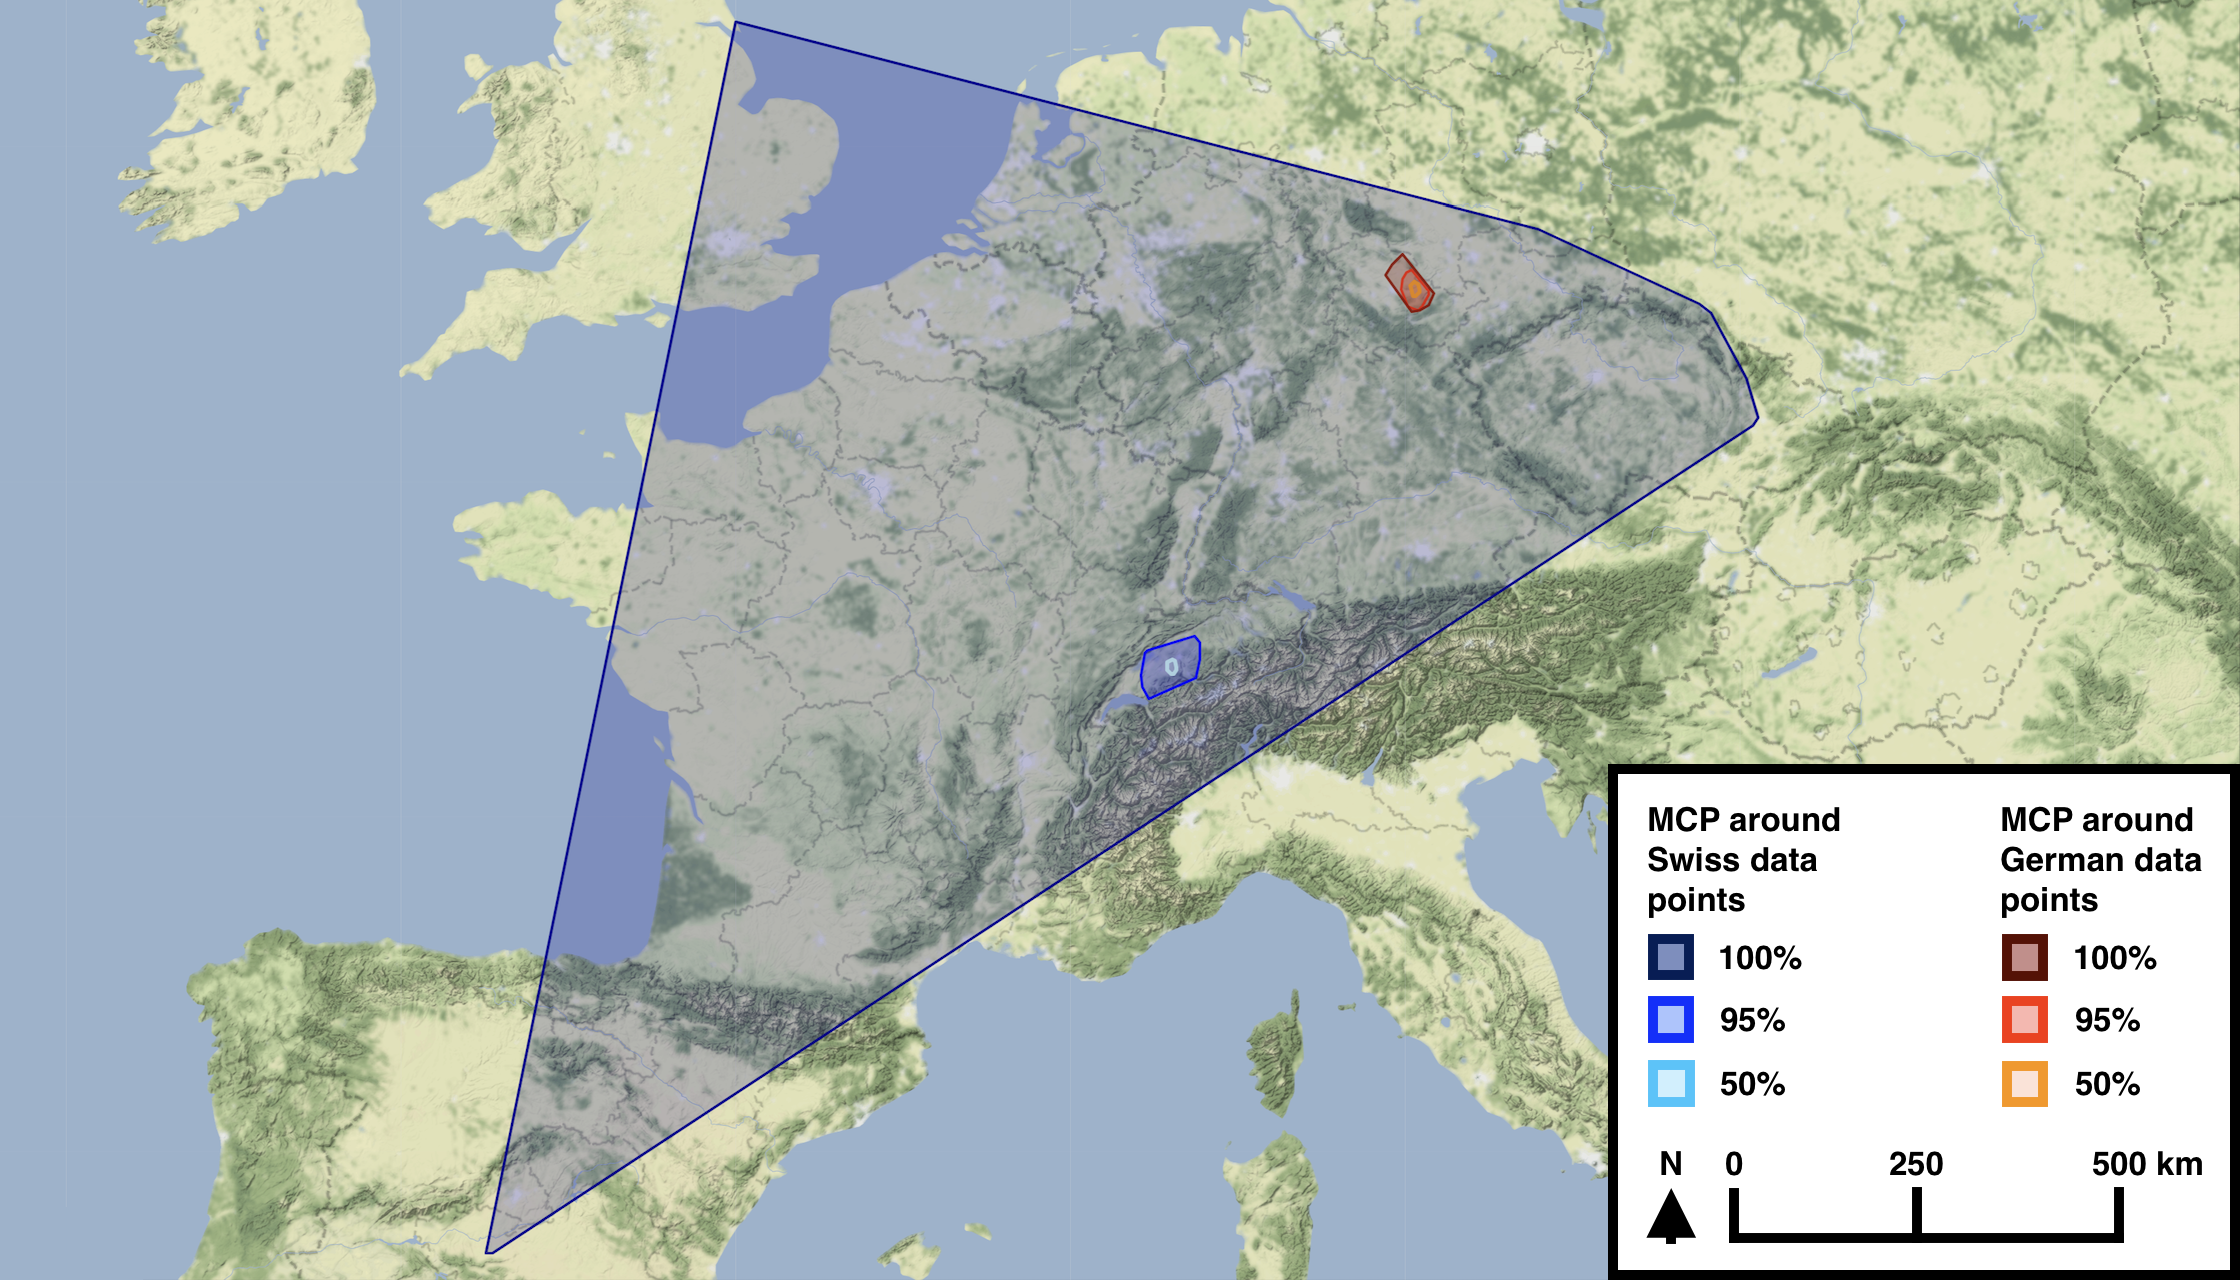
\includegraphics[width=1\textwidth]{figures/maps/All_data_MCP.png}
\caption[MCP (100\%, 95\% \& 50\%) around all red kite GPS locations of Switzerland and Germany during the breeding cycle]{MCP (100\%, 95\% \& 50\%) around all red kite GPS locations of the Swiss Ornithological Institute (blue) and all red kite locations contributed by Thomas Pfeiffer (red) during the breeding cycle. Base map: Stamen.}
\label{figure:map_breeding_area}
\end{figure}



\subsection{Pre-Processing} \label{subsection:preprocessing}
Locations without timestamps or coordinates were deleted, as well as duplicates. The dataset was reduced to the period from 1 February to 15 August to fully cover the  breeding period of red kites \parencite{aebischer2021rotmilan}. Spatial outliers were eliminated by only considering data in Europe with a buffer of 100 kilometres corresponding to the distributional range of red kites \parencite{garcia2022seasonal, literak2022disperal, mougeot2011breeding, panter2022age, seoane2003effects}. Temporal outliers were deleted, which could be defined by velocities between consecutive locations that exceed realistic flight speeds of red kites \parencite{garcia2022seasonal}. GPS locations were resampled to a temporal resolution of one-hour intervals to account for differences in sampling regime and divided into bursts. A burst is defined as a sequence of consecutive locations of the same bird that does not have a gap. Only bursts with a minimum of three locations were considered. Finally, the data was transformed from WGS84 (EPSG: 4326) to the equidistant ETRS89-extended (EPSG: 3035), to calculate realistic distance measures.



\subsection{Home Range Detection} \label{subsection:homerange}
For the detection of the home range, only data during the months of February, March, April and May were considered, as red kites occupy their home range during this period. Birds with less than 14 days of data were removed, because the algorithm requires two weeks of data to detect a potential settlement.

To determine whether a bird has occupied a territory, two parameters were used. Firstly, the area used by the individual was determined, as this can provide information about whether a bird has settled in a territory or not. Red kites reduce the spatial range of their movements upon establishing a home range containing a potential breeding site and resources \parencite{spatz2022sex}. Furthermore, the spatial displacement of the calculated area was also analysed to exclude cases where an individual may have a small home range but constantly relocates to a different area and thus, cannot have settled in a territory. To find suitable thresholds for the parameters used, the breeding data based on observations were used (Red Kite Project of the Swiss Ornithological Institute).

To calculate the home range area, 95\% MCP was used, since a rough guide value of the actual home range is sufficient for the detection of a home range in this work, and MCP is easier to parameterise than other home range detection methods. Calculating 95\% MCPs to define home ranges is a common arbitrary standard in movement ecology \parencite{fieberg2007kernel, hasselblad2007male, kernohan2001analysis, laver2008critical, signer2021fresh}. This approach saves a lot of computing power compared to more advanced metrics, yielding comparable results. To calculate the spatial displacement, the centoids of the MCPs were calculated, which then allows distance determinations between the calculated MCPs. Both parameters were calculated with the R package \textit{amt} by \textcite{signer2019amt}.

To determine the moment of settlement in time, an MCP was calculated for each bird and week. Then, with the expectation that the home range of most birds will decrease with a settlement, a threshold was identified for the MCP area below which a settlement can be assumed. Values from 10 to 100 km$^2$ were tested in steps of 10. Since a settlement cannot be assumed if only one week meets the requirement, the number of consecutive weeks that fall below the tested area values was calculated. The appropriate MCP area value combined with the optimal number of consecutive weeks was then determined by means of a visual change point detection (Figure~\ref{figure:hr_area_weeks}). The analysis showed that the threshold values of an MCP area of below 60~km$^2$ for at least 3 consecutive weeks must be met for settlement in a home range to be possible. In a final step, in order to remove birds that fulfilled the previous requirements but shifted their home range each week, a threshold value for centroid displacement was determined, which must not be exceeded for a settlement to be assumed. This distance value was also visually identified using a change point detection (Figure~\ref{figure:centroid_displacement}). The analysis showed that the minimum displacement of the calculated home ranges for all consecutive weeks in which they meet the area requirement must not exceed 760~m.

For all 908 cases for which a home range detection was carried out, the differences between the two categories (whether a home range was occupied or not according to the validation data) were analysed regarding both the number of consecutive weeks spent in an area of less than 60 km$^2$ and the centroid displacement between the respective areas. In addition, the difference between the sexes was examined.

\begin{figure}[H]
\centering
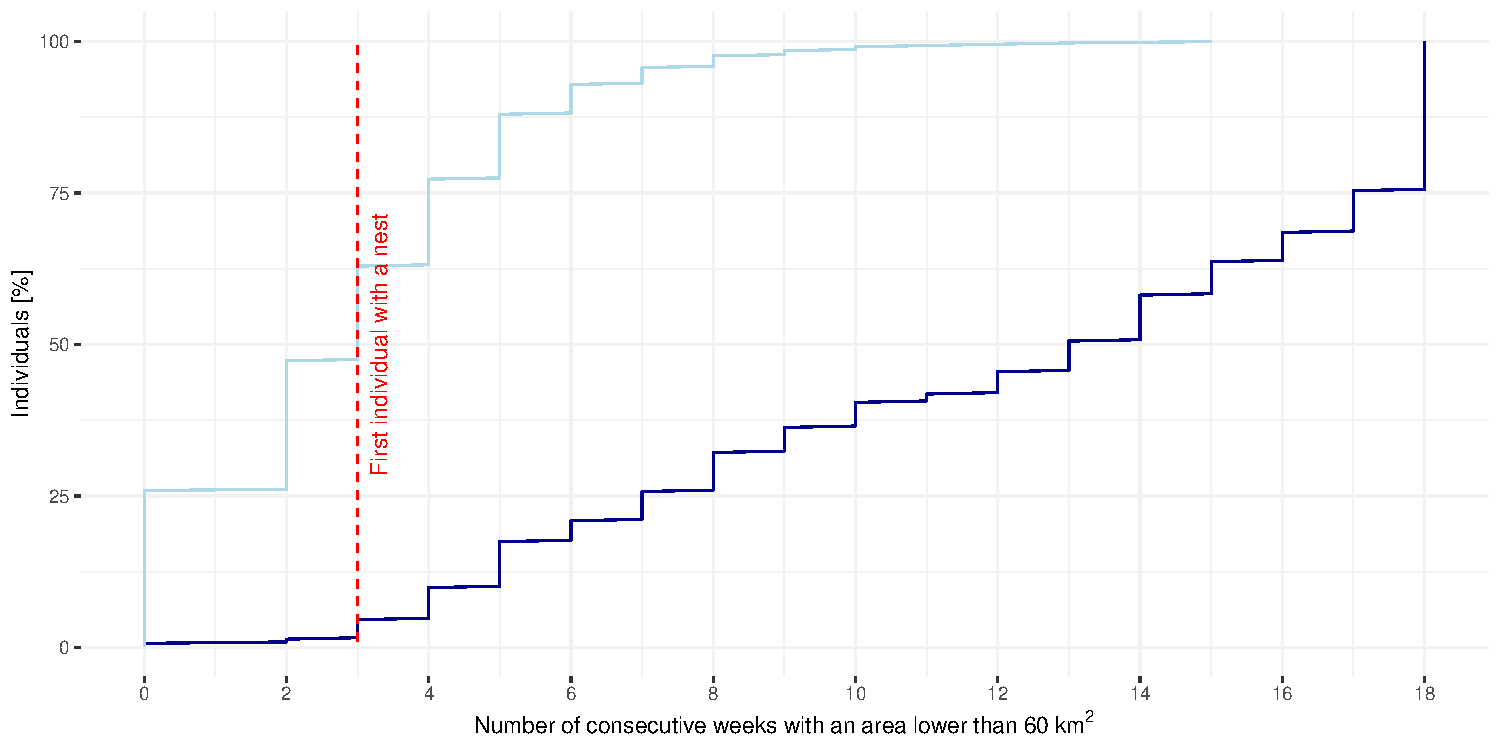
\includegraphics[width=1\textwidth]{figures/methods/01_size_60consecutive.pdf}
\caption[Change point detection for the number of weeks with an MCP < 60~km$^2$]{Visual analysis of a change point detection for the number of consecutive weeks where the MCP area is smaller than 60~km$^2$. Different colours depict the two categories of birds (dark blue = home range, light blue = no home range). The dashed red line shows the lowest number of consecutive weeks for a bird with a nest, which indicates the threshold value to filter out the highest possible number of individuals without a home range, while retaining all the individuals with a home range.}
\label{figure:hr_area_weeks}
\end{figure}

\begin{figure}[H]
\centering
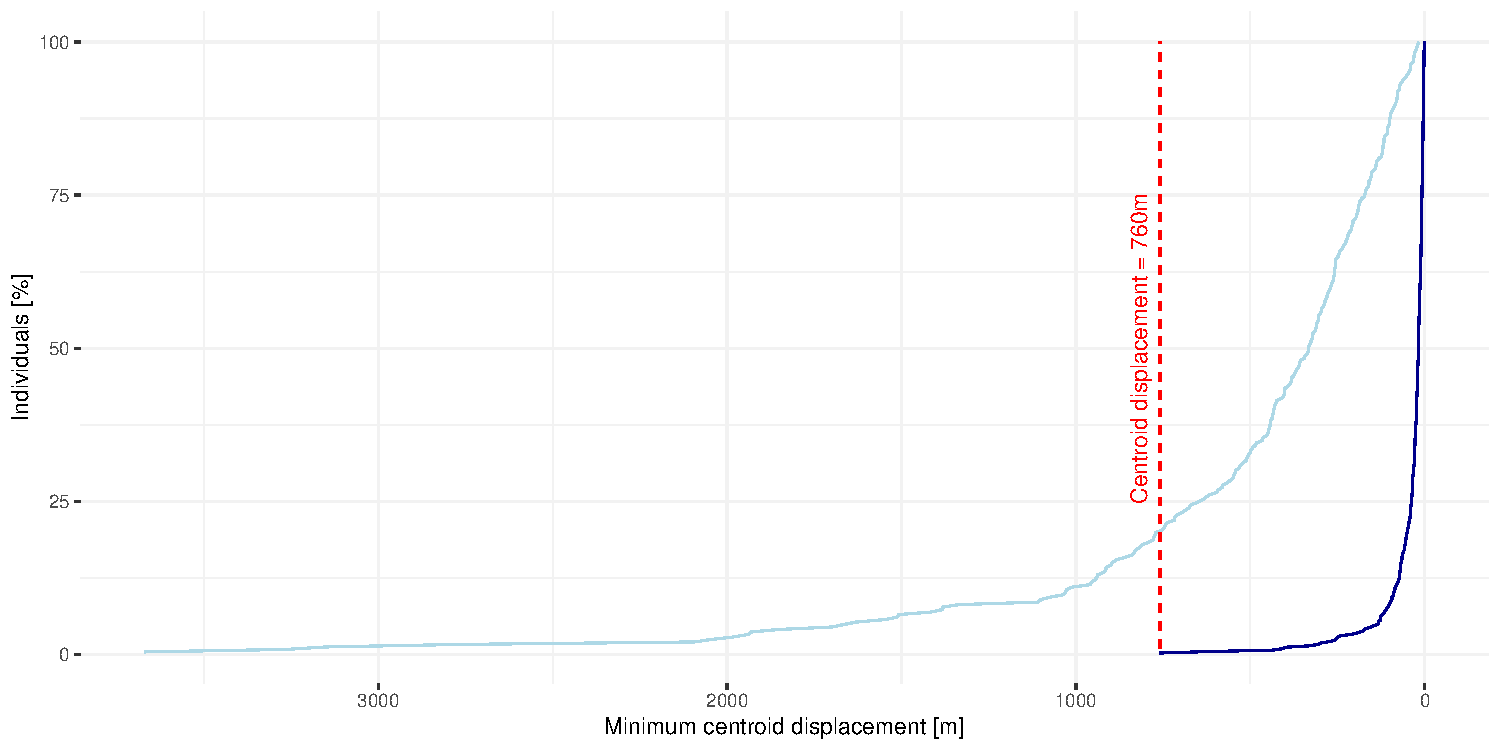
\includegraphics[width=1\textwidth]{figures/methods/03_centroid_displacement.pdf}
\caption[Change point detection for the minimum centroid displacement between weeks from a settlement onwards]{Visual analysis of a change point detection for the minimum centroid displacement between weeks from a settlement onwards. Different colours depict the two categories of birds (dark blue = home range, light blue = no home range). The dashed red line shows the threshold value that filters out the highest possible number of individuals without a home range, while retaining all the individuals with a home range.}
\label{figure:centroid_displacement}
\end{figure}



\newpage
\subsection{Nest Detection} \label{subsection:nest}
The aim of the nest detection is firstly to find out for all individuals whether they have a nest or not, and secondly to locate the potential nest. Only data during the months of March, April, May and June were considered, as this is the core phase of breeding when all breeding individuals are expected to be in the vicinity of the nest \parencite{aebischer2021rotmilan}. Although there are individuals that are at the nest much earlier, there are also those that are still in their wintering area in February. As a result, there are cases where birds repeatedly visit the same place, for example a feeding site, in their wintering area. When these birds later breed in their breeding area, the lack of sunlight under the canopy and the long time spent in the nest can lead to missing GPS data. As a result, the frequently visited site in the actual wintering area could then be wrongly identified as a nest due to the availability of more data. To avoid this particular case, the data in this step are only taken into account from March onward. In the later summer months, the same behaviour can lead to the same error, which is why these months are also not considered, as nest building in July and later are unlikely. Furthermore, for each bird individually, the data before the first week in which it settled in its home range were deleted, as territory occupation was assumed a prerequisite to nest building. For nest detection, it was also important to remove the locations recorded during the night and during twilight. The purpose of this step was to eliminate locations away from the actual nest. Especially at the beginning of the breeding phase, while the nest is still being built, some birds tend to spend the night at a roosting place which they share with other red kites \parencite{aebischer2021rotmilan}. This revisited site could easily be mistaken for the actual nest location. The night locations were calculated with the function \textit{time\_of\_day} of the R Package \textit{amt} by \textcite{signer2019amt}.

To determine whether a bird has a nest, revisitations and residence time were calculated for each GPS position using the R package \textit{recurse} by \parencite{bracis2018revisit}, as the nest is the place that is naturally visited the most during the breeding period. To find suitable thresholds for the parameters used, the validation data of the Swiss Ornithological Institute were used.

Using the function \textit{getRecursions}, the movement trajectory for each red kite and each year was analysed. With a buffer of 50~m, the number of revisitations and residence time were calculated for each point of the trajectory. The buffer size of 50~m was chosen because the radius should not be much smaller than most distances between locations and should also be larger than the measurement error \parencite{bracis2018revisit}.

Highly frequented sites do not necessarily represent an actual nest. Non-breeding individuals that have not occupied a home range may move over large areas but still frequent certain locations. Breeding individuals, on the other hand, stay mainly in the vicinity of the nest, which is why an accumulation of highly frequented sites around the nest location is expected to be seen in the data. In order to localise the area around the nest and to exclude possible frequently visited sites before and after breeding, the area covered by the most visited sites was calculated for each individual. The optimal number of most visited locations and the size of the area they cover were the subject of a further visual change point detection (Figure~\ref{figure:nest_area_45}). The analysis showed that the threshold values of 45 most visited locations, covering an area of less than 0.052~km$^2$, were the most suitable for distinguishing individuals with a nest from individuals without one.

From the remaining individuals, the potential nest site was then determined. The most visited location was assumed to be the nest site. If several locations had the same value, the one with the longest residence time was chosen.

In order to find out whether the most visited location was sufficiently visited and enough time was spent there to represent a nest, a second revisitation analysis was carried out. This time, the revisitation analysis focused on the predicted nest location with a buffer radius of 50 metres. The function \textit{getRecursionsAtLocations} was used for this purpose. For each day it was calculated how often the predicted nest location was visited and how much time was spent there. From this, a relative value for the average daily revisitations and the average daily residence time was calculated over the entire period in which data were available. Suitable threshold values that must be reached were again selected by means of a visual change point detection (Figure~\ref{figure:revisits_cpd}~and~\ref{figure:residence_time_cpd}). The analysis showed that the most frequently revisited locations must be revisited at least 0.54 times per day and for at least 31 minutes per day to represent a potential nest.

For all 624 cases for which a nest detection was carried out, the differences between the two categories (whether a nest was present or not according to the validation data) were analysed regarding residence time and revisitations. In addition, the difference between the sexes was examined.

\begin{figure}[H]
\centering
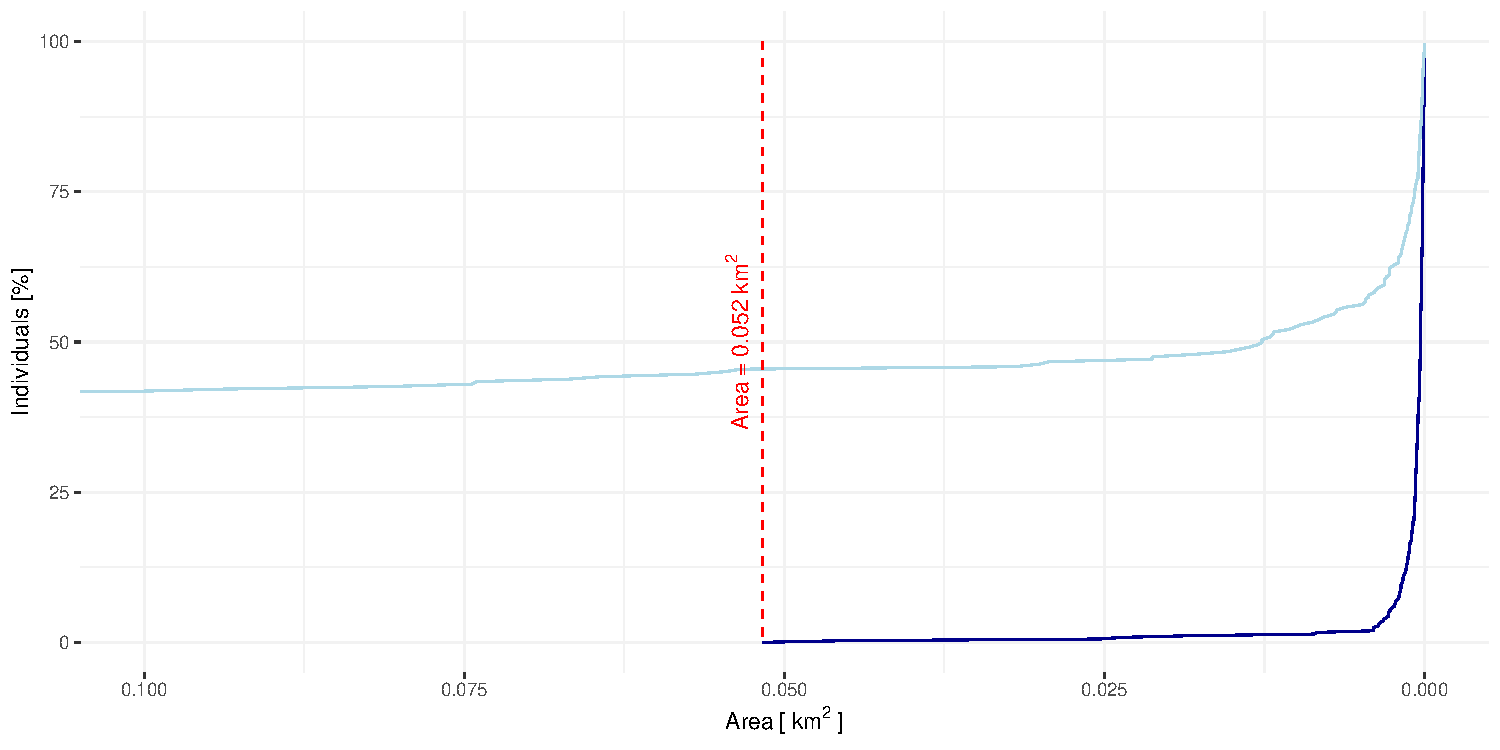
\includegraphics[width=1\textwidth]{figures/methods/01_area_45_most_visited.pdf}
\caption[Change point detection for the size of the area of the 45 most visited locations]{Visual analysis of a change point detection for the size of the area of the 45 most visited locations. Different colours depict the two categories of birds (dark blue = home range, light blue = no home range). The dashed red line shows the highest area value for a bird with a nest, which indicates the threshold value to filter out the highest possible number of individuals without a nest, while retaining all the individuals with a nest.}
\label{figure:nest_area_45}
\end{figure}

\begin{figure}[H]
\centering
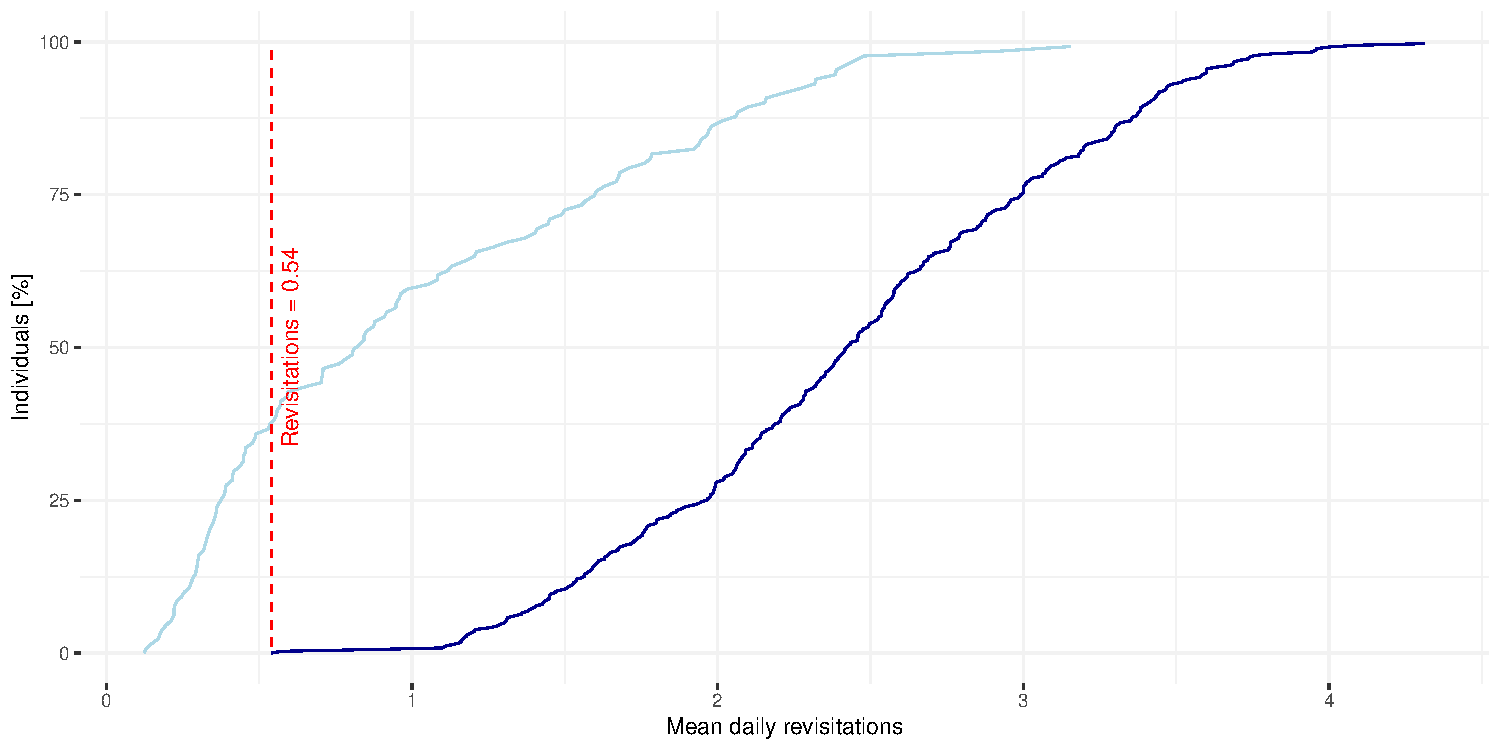
\includegraphics[width=1\textwidth]{figures/methods/06_revisits.pdf}
\caption[Change point detection for the mean daily revisitations at the predicted nest location]{Visual analysis of a change point detection for the mean daily revisitations at the predicted nest location. Different colours depict the two categories of birds (dark blue = home range, light blue = no home range). The dashed red line shows the lowest number of mean daily revisitations for a bird with a nest, which indicates the threshold value to filter out the highest possible number of individuals without a nest, while retaining all the individuals with a nest.}
\label{figure:revisits_cpd}
\end{figure}

\begin{figure}[H]
\centering
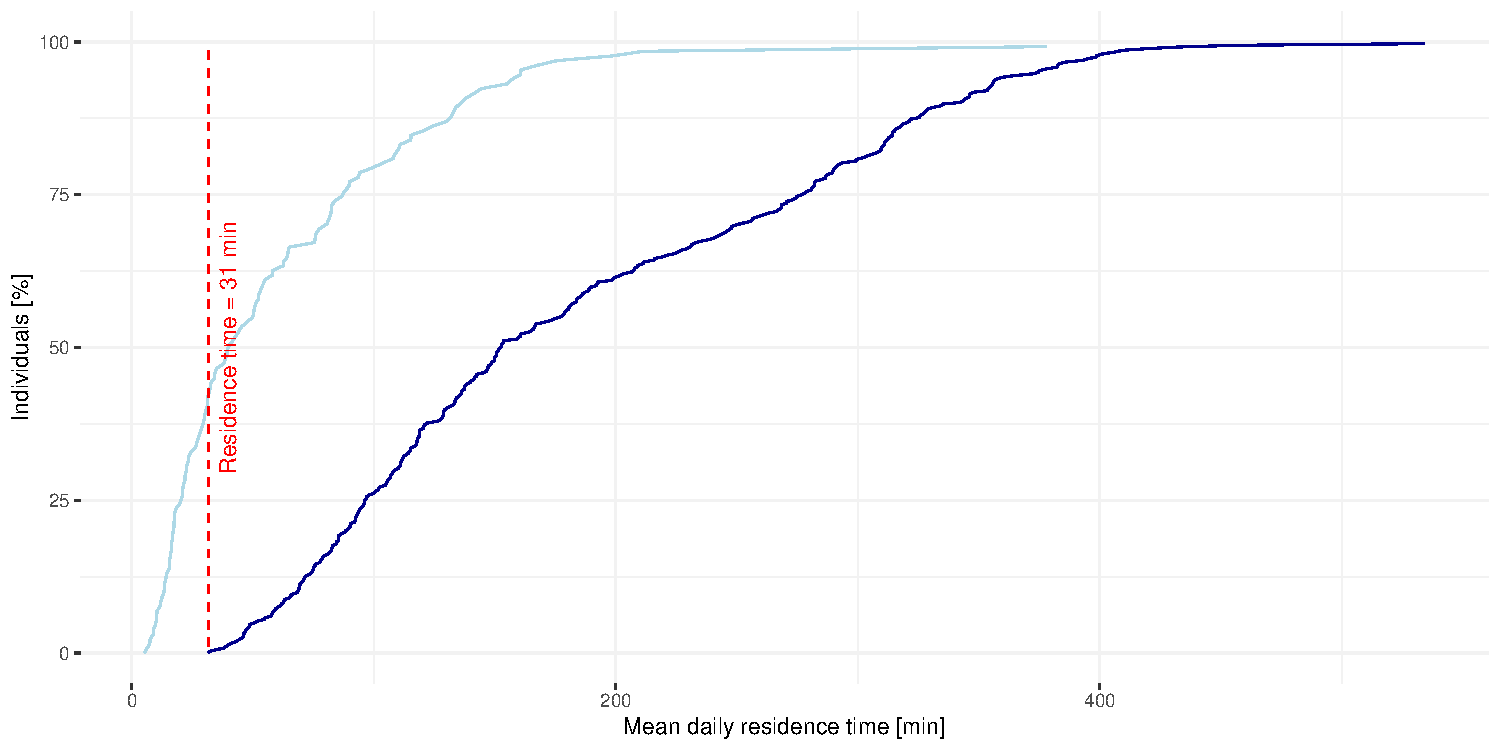
\includegraphics[width=1\textwidth]{figures/methods/04_residence_time.pdf}
\caption[Change point detection for the mean daily residence time at the predicted nest location]{Visual analysis of a change point detection for the mean daily residence time at the predicted nest location. Different colours depict the two categories of birds (dark blue = home range, light blue = no home range). The dashed red line shows the lowest mean daily residence time for a bird with a nest, which indicates the threshold value to filter out the highest possible number of individuals without a nest, while retaining all the individuals with a nest.}
\label{figure:residence_time_cpd}
\end{figure}



\subsection{Brood Phase Identification} \label{subsection:brood_phase_identification}
The aim of the brood phase identification is to identify the two phases of incubating the eggs and feeding the nestlings during a brood cycle. The duration of these two phases is then used to distinguish successful broods from unsuccessful broods.

To detect the two phases of incubating and feeding, the aim was to predict separately for each day of a brood cycle whether an individual was incubating, feeding or not breeding (this last category will from here on be referred to as non-breeding). To classify a day into one of the three categories, the probability of classification into each of the categories should be calculated for the movement pattern on that day. The percentages of the different categories on a day would then make it possible to classify the day into one of the categories. Calculating probabilities instead of assigning the day directly to a category offers the advantage that with breeding biology background knowledge, the categories can be meaningfully classified through an interpretation of the predictions or a rule-based approach.

There are numerous classification methods that allow daily movement patterns to be assigned to one of the three categories mentioned. For the sake of simplicity, only the chosen method is explained here, highlighting its specific advantages. The approach of using a multinomial logistic regression model (MLRM) was chosen, which is characterised by the fact that, compared to a binomial logistic regression model, the response variable is defined in more than two non-ordinal categories \parencite{kwak2002multinomial}. This approach can be particularly advantageous as it means that there is no need to collapse several categories in order to use the widely used and more familiar binomial logistic regression model \parencite{kwak2002multinomial}. The MLRM was generated with the R package \textit{brms} by \textcite{buerkner2017brms}. The package \textit{brms}, allows to use Bayesian multilevel models in R based on the probabilistic programming language \textit{Stan}. The advantage of the Bayesian implementation is the fact that it is based on probability distributions, which is particularly suitable for this work, as it allows probabilistic predictions and a final interpretation of the predictions.



\subsubsection{Data Pre-Processing for the MLRM} \label{subsubsection:mlrm_preprocessing}
To train the MLRM, only data from 10 March until 31 July were considered, as this is the period in which the entire brood cycle of the vast majority of red kites takes place. In western Switzerland, no start of breeding has yet been observed before 14 March \parencite{scherler2023brutbiologie}. The date was rounded off to 10 March to create a buffer for unexpected special cases. By the end of July, basically all the young birds have fledged \parencite{aebischer2021rotmilan}. To ensure that the model was created with a sufficiently detailed dataset, the data were subjected to further requirements. Firstly, the individuals considered had to provide at least one day of data in each of the months considered. Secondly, days with less than three GPS locations were filtered out, as this is the minimum requirement for calculating an area. Finally, the number of days (143) was multiplied by three locations, which was then used as the minimum number of GPS locations that must be present over the entire period (429). In addition, sufficient validation data had to be available on the duration of incubation and feeding or the date of egg laying, the hatching date and the date when the young birds left the nest. This resulted in a dataset of 222 brood cycles from 102 individuals with sufficient data and information. Exactly half of the breeding cycles stem from females and the other half from males.

The response variable of the MLRM is the brood phase, which is predicted on a daily basis and has three categories: breeding, feeding and non-breeding. Several explanatory variables were calculated that could be suitable for integration into the MLRM from a biological perspective. All variables were calculated on a daily basis to meet the model's requirement to calculate predictions on a daily basis. The explanatory variables calculated were 95\% MCP, revisitation at the nest location, residence time at the nest location, distance to the nest location, and step length between GPS locations. MCPs and step lengths were calculated with the R package \textit{amt} by \textcite{signer2019amt}, revisitations and residence time with the R package \textit{recurse} by \textcite{bracis2018revisit} and distance to the nest location with the R package \textit{sf} by \textcite{pebesma2018simple}. In addition, the two movement-independent variables sex and sensor temperature were included. Sex was included due to the different roles of the parents during the brood cycle \parencite{spatz2021zwischen}, while the body temperature of females was expected to increase during breeding \parencite{aebischer2021rotmilan}. Finally, the number of GPS locations per day was defined as a control variable and an ID combining the individual and the respective year as a random effect. The number of GPS locations per day was included in the model as it was assumed to influence the accuracy of the calculation of movement patterns. The ID combining the individual and the respective year was integrated to correct for dependencies of the data, as an individual can provide data over several years.

For most variables, several variations were calculated in order to analyse which were most suitable for the final model. For step length, distance to the nest location and temperature, the daily mean, minimum and maximum values were calculated. For 95\% MCP, revisitations, residence time, distance to the nest, step length and temperature, moving average values were calculated over the previous three, five and seven days (including the day under consideration). This eliminates outliers that can be caused by individual days in which the movement behaviour deviates from the expected behaviour or the data is insufficient. For example, movement behaviour can be strongly influenced by extreme weather conditions, so that the red kites only perch at the nest during a day in order to protect their nestlings and not endanger themselves, while they would actually search for food in normal weather conditions \parencite{aebischer2021rotmilan}.

As a final step, all variables were scaled and centered. Besides the fact that this prevents convergence problems in linear models, it also makes the model applicable to other red kite populations with different dimensions of movement.



\subsubsection{Implementation of the MLRM} \label{subsubsection:mlrm_implementation}
The dataset with 222 brood cycles was divided into a training dataset (70\%, 155 brood cycles, 76 females and 79 males) and a test dataset (30\%, 67 brood cycles, 35 females and 32 males). With the developed variations of the variables (Section~\ref{subsubsection:mlrm_preprocessing}), different MLRMs were developed and trained with the training dataset.

In order to determine the most appropriate variation of each variable as explanatory variable, identical models were developed using a different variation of each variable. To determine the most appropriate variation, estimates of the variables were plotted. For each variable, it was visually determined which variation had the strongest influence on the model. The respective variation was then selected to further generate the best performing model. The variables that did not show large estimates in all variants were excluded from the further models. The variations of the explanatory variables that were ultimately used for the model are listed in Table~\ref{table:mlrm_variables}.

With the appropriate explanatory variables, several variants of models were developed in which different interactions between the variables were built in and the variables were weighted differently. This resulted in 17 different models, which were then compared with each other in terms of their performance. To compare the models with each other, the efficient approximate leave-one-out (LOO) method was used. LOO is used for cross-validation of Bayesian models. The method is implemented in the R Package \textit{brms} and is based on the description of \textcite{vehtari2017practical}, who present an efficient computation of LOO using on Pareto-smoothed importance sampling.

The best performing model included sensor temperature as an explanatory variable. However, a simpler model without sensor temperature performed similarly (the later predictions with the test dataset showed also similar results). Finally, the model without sensor temperature was selected as the appropriate model for two reasons. On the one hand, the sensor temperature is a mixed temperature of the air temperature and the body temperature. The two proportions differ according to sensors, activity of the bird, weather and season, which complicates the interpretation of the temperature. On the other hand, there are GPS transmitters without temperature sensors, for which the model can also be used. Thus, the MLRM is applicable to a wider range of data, especially older data. Due to a similar performance, the model with the fewest possible variables and consistent performance was chosen. A summary of the MLRM is shown in Appendix~\ref{appendix:mlrm_formula}. To analyse the performance of the model in terms of predictions, it was applied to the test dataset. The visual representations of the predictions of all 67 brood cycles are listed in Appendix~\ref{appendix:mlrm_predictions_test}.

\begin{table}[H]
\begin{center}
\caption[Explanatory variables of the MLRM]{Explanatory variables that were integrated in the MLRM.}
\label{table:mlrm_variables}
\begin{tabular}{| p{6cm} | p{2.5cm} | p{2.5cm} |}
\cline{1-3}
\textbf{Variable description} & \textbf{Variable type} & \textbf{Variable \newline range/levels} \\
\hline
95\% MCP \newline (moving average over 7 days) & Numeric & 0.0000003 - 1\\ 
\hline
Revisitations at nest location \newline (moving average over 7 days) & Numeric & 0 - 1 \\
\hline
Residence time at nest location \newline (moving average over 7 days) & Numeric & 0 - 1\\
\hline
Daily mean distance to nest location \newline (moving average over 7 days) & Numeric & 0.00008 -1\\
\hline
Sex & Binary & 0, 1\\
\hline
\end{tabular}
\end{center}
\end{table}



\subsubsection{Brood Success Evaluation}
In order to derive the breeding success from the raw model predictions, three approaches were used. In all three approaches, the model predictions are compared with the shortest known brood duration for this species. According to \textcite{aebischer2021rotmilan}, red kites must be incubating at least 28 days and feeding the nestlings at least 42 days in order to successfully produce fledged offspring. If an individual reached the minimum number of days in the year under consideration, it was classified as a successful brood in all three approaches.

\vspace{1\baselineskip}
\noindent \textbf{Raw Model Predictions} \newline
\noindent In this approach, the category of a day is derived directly from the raw model prediction. Every day is classified in the category that shows the highest probability value on the respective day.
The days of the respective category are then added up. When the minimum number of days per category was reached, the brood was considered successful. A visual representation of the raw model predictions compared to the validation data from the field observations can be seen in Figure~\ref{figure:example_prediction} (left).

\vspace{1\baselineskip}
\noindent \textbf{Merged Categories} \newline
\noindent In this approach, the two categories incubating and feeding are merged into a new category "breeding". Thus, there are only the two possibilities that an individual is breeding or non-breeding. This method is based on the idea that movement behaviour patterns during incubation and during feeding are similar (especially in male red kites), making these two categories easy to misclassify, but still clearly distinguishable from non-breeding. A day is categorised as non-breeding as soon as the probability is above 50\% and as breeding if the probabilities of the two categories incubating and feeding add up to at least 50\%. When the number of breeding days reach the minimum number of days of incubating and feeding combined (70 days), the brood was considered successful.

\vspace{1\baselineskip}
\noindent \textbf{Rule-Based Adaptation} \newline
\noindent In this approach, the raw model predictions were adjusted using rules based on biological knowledge on the respective breeding phase. The application of the rules is to ensure that the predictions are smoothed and outliers in the calculated movement behaviour that do not fit the expected pattern are corrected. While the predictions were manipulated, it was intended not to bias the predictions too much to match expected patterns and thus potentially distort the result. The following rules were used for this approach:

\begin{itemize}
    \item The first day of incubation must not be isolated. There have to be at least five days of incubation in a row. All previous days are reclassified to non-breeding.
    \item The last day of incubation must be no later than 39 days after the first day of incubation. All later days of incubation are reclassified to feeding.
    \item Between the first day of incubation and the last day of incubation, isolated days of feeding are reclassified to incubating.
    \item The first day after the last day of incubation is reclassified to feeding.
    \item The last day of feeding must be no later than 50 days after the first day of feeding. All later days of feeding are reclassified to non-breeding.
    \item Between the first day of incubation and the last day of feeding, single isolated non-breeding days are reclassified to the category they are located in.
\end{itemize}

\noindent A visual example of the influence of this rule-based adaptation approach on the model predictions can be seen in Figure~\ref{figure:example_prediction} (right).

\begin{figure}[H]
\centering
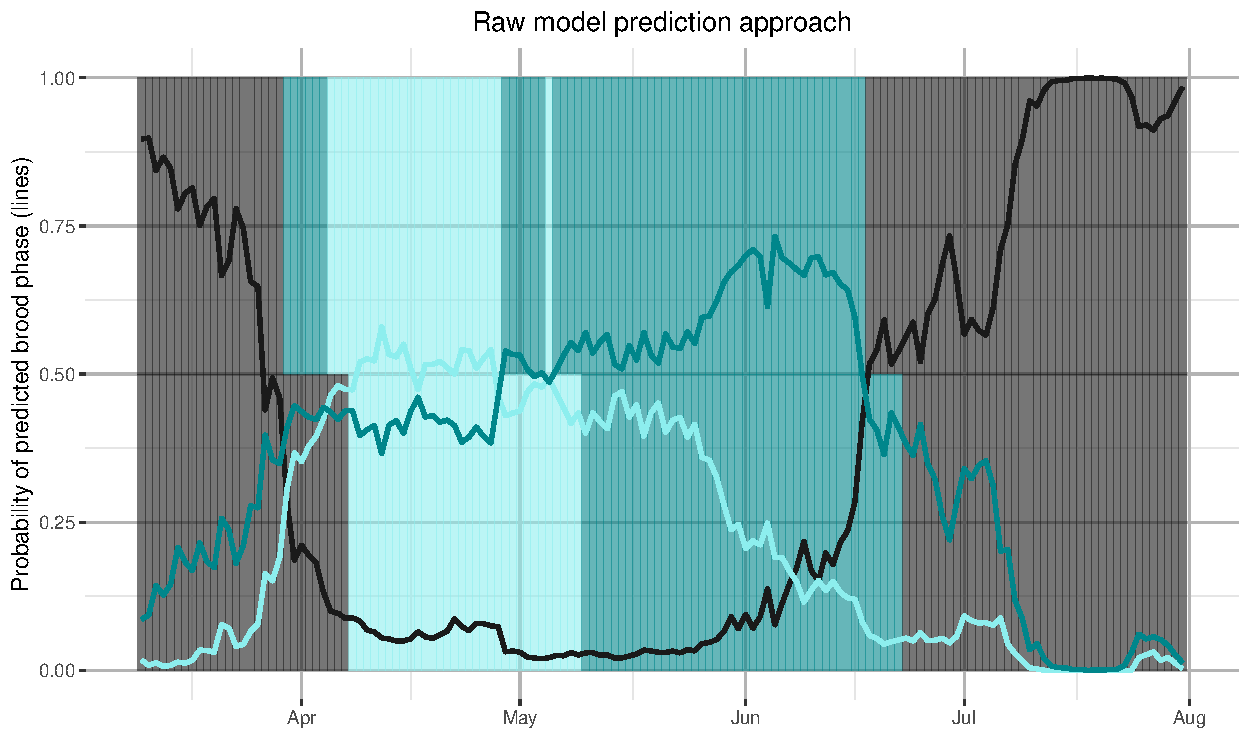
\includegraphics[width=0.45\textwidth]{figures/methods/07_prediction_example_raw.pdf}
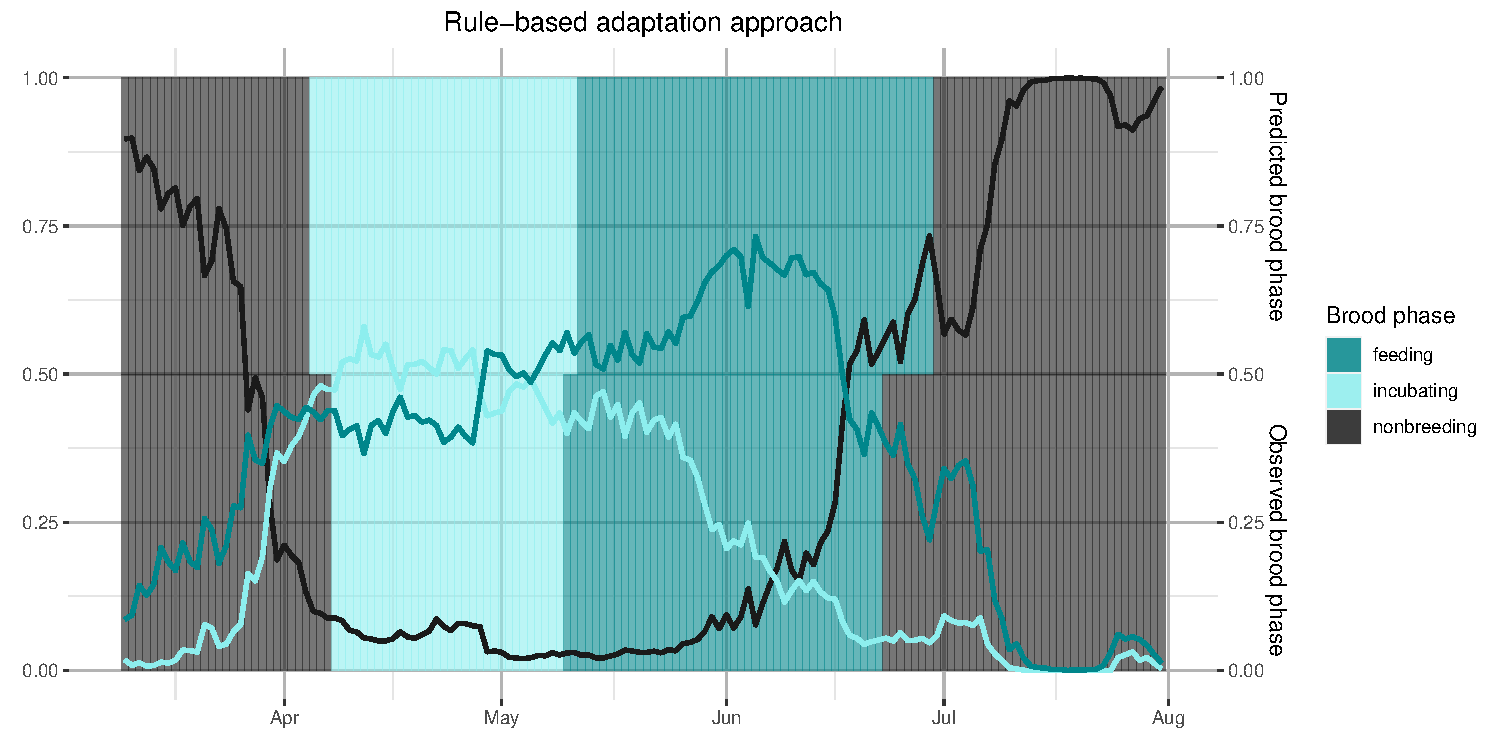
\includegraphics[width=0.54\textwidth]{figures/methods/08_prediction_example_rule.pdf}
\caption[Example of an MLRM prediction]{Example of the model predictions for an individual. The lines show the calculated probability for one of the three categories (light blue = incubating, turquoise = feeding, grey = non-breeding). The bars in the lower half of the plot show the actual breeding behaviour based on field observation data, while the bars in the upper half show the predicted category. The predictions based on the raw model prediction approach (left) are compared to the predictions based on the rule-based adaptation approach (right).}
\label{figure:example_prediction}
\end{figure}



\subsubsection{Validation of Brood Phase Identification}
Finally, the model was validated with two different datasets.

On the one hand, there were FP cases that remained after the two steps of home range detection (Section~\ref{subsection:homerange}) and nest detection (Section~\ref{subsection:nest}). These individuals were assigned a nest even though they did not breed at all. With the data of these individuals, the performance of the MLRM could be validated on non-breeding red kites. This step served to investigate whether the model reliably recognises non-breeding individuals as such and does not misinterpret their movement behaviour as breeding behaviour.

On the other hand, the model was applied to the movement data of the 28 successfully breeding adults in Thuringia provided by Thomas Pfeiffer. With the data of these individuals, the performance of the model could be validated on movement data from other geographical regions. This step served to investigate whether the scaling and centering of the variables allows a reliable application of the model to individuals with different scales of movement behaviour.